\documentclass[../main.tex]{subfiles}
\graphicspath{{\subfix{../images/}}}

\begin{document}


The problem of assigning a class to grey-scale images of clothing 
came with some difficulties.
Considering the different complexity of the three models 
that we implemented, we still see the same trends in the predictions.


\subsection{Class Overlap}

One of the main challenges all the models faced with the Fashion MNIST 
data set, was class overlap. As mentioned earlier, our feed-forward 
neural network wrongly classified class $4$ (Shirt) as class $0$ (T-
shirt/top) and class $2$ (Pullover). Taking a look at 
all the confusion matrices for the three classifiers, we see an 
evident tendency that class $4$ (Shirt) is misclassified. This is 
also what we expected since the three items of clothing are visually 
quite similar, which explains the class overlap we discovered. When 
we compare that to class $1$ (Trouser) which are a more unique 
type of clothing, it is easier for the models to distinguish, this is 
also depicted clearly in all of the confusion matrices.

\begin{figure}[ht]
    \centering
    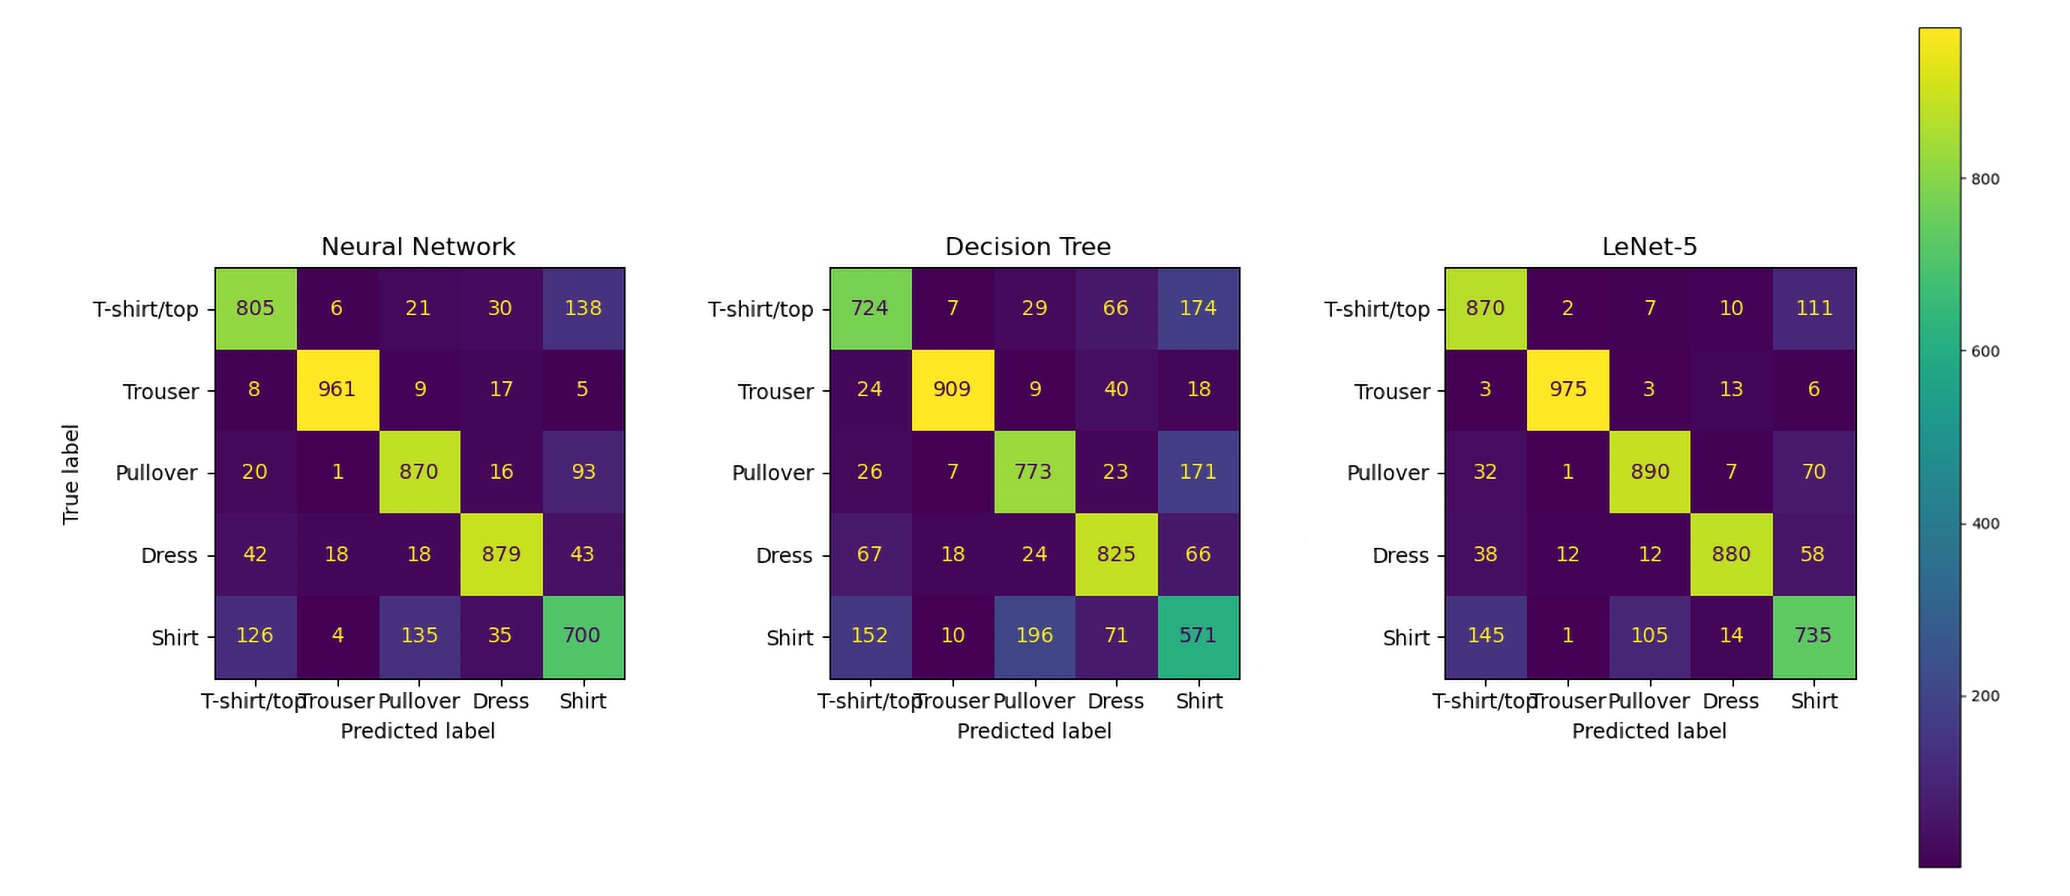
\includegraphics[width=\textwidth]{all_classifiers_confusion_matrix}
    \caption{Confusion matrices for all classifiers}
    \label{fig:all-confusion-matrices}
\end{figure}


\subsection{Model Comparison}

Decision trees and tree-based approaches in general, are typically 
not as competitive as other machine learning approaches in terms of 
accuracy \autocite{JamesStatisticalLearning}. 

The advantage of using a decision tree classifier is that it is a 
highly interpretable model and it is possible to visualise each 
decision. Furthermore it has a shorter training time than other 
machine learning methods since the tree is usually built with 
a top-down greedy approach. 
However, with the given classification problem at hand the 
interpretability the model provides is not as useful compared to 
other situations. First of all, we are training the model on 
principal components, already at this point we are loosing a lot 
of interpretability. 
If we were to train on the original data set, we 
would still lack interpretability since the features are low-level 
features. 

If interpretability is not attainable or desirable, more complex 
models can be used.
For such highly complex data sets, like the Fashion MNIST data set, 
a better suited model for classification is a feed-forward 
neural network. Feed-forward neural networks are excellent at 
solving complex classification problems compared to simpler models, 
and therefore we get a better performance than our decision tree. 
Nevertheless, feed-forward neural networks are not able to capture 
the locality of features. 
Convolutional neural networks, on the other hand, are built for 
image analysis. They are able to process image data in two and three-
dimensions with the help of convolutional and pooling layers. 
This is a big advantage over the other two models since both are 
only able to handle one-dimensional data.
This is likely also a reason why our results for the 
convolutional neural network are better than the other two models.


\end{document}